\subsection{Implementation}
Our networks and loss functions are implemented using built-in TensorFlow \cite{TensorFlow}
functions, enabling us to use automatic differentiation for all gradient
computations. To make our code easy to extend and flexible, we build on
the TensorFlow Object detection API \cite{TensorFlowObjectDetection}, which provides a Faster R-CNN baseline
implementation.
On top of this, we implemented Mask R-CNN and the Feature Pyramid Network (FPN)
as well as extensions for motion estimation and related evaluations
and postprocessings. In addition, we generated all ground truth for
Motion R-CNN in the form of TFRecords from the raw Virtual KITTI
data to enable fast loading during training.
Note that for RoI extraction and cropping operations,
we use the \texttt{tf.crop\_and\_resize} TensorFlow function with
interpolation set to bilinear.

\subsection{Datasets}
\label{ssec:datasets}

\paragraph{Virtual KITTI}
The synthetic Virtual KITTI dataset \cite{VKITTI} is a re-creation of the KITTI
driving scenario \cite{KITTI2012, KITTI2015}, rendered from virtual 3D street
scenes.
The dataset is made up of a total of 2126 frames from five different monocular
sequences recorded from a camera mounted on a virtual car.
Each sequence is rendered with varying lighting and weather conditions and
from different viewing angles, resulting in a total of 10 variants per sequence.
In addition to the RGB frames, a variety of ground truth is supplied.
For each frame, we are given a dense depth and optical flow map and the camera
extrinsics matrix. There are two annotated object classes, cars, and vans (N$_{cls}$ = 2).
For all cars and vans in the each frame, we are given 2D and 3D object bounding
boxes, instance masks, 3D poses, and various other labels.

This makes the Virtual KITTI dataset ideally suited for developing our joint
instance segmentation and motion estimation system, as it allows us to test
different components in isolation and progress to more and more complete
predictions up to supervising the full system on a single dataset.

For our experiments, we use the \emph{clone} sequences, which are rendered in a
way that most closely resembles the original KITTI dataset. We sample 100 examples
to be used as validation set. From the remaining 2026 examples,
we remove a small number of examples without object instances and use the resulting
data as training set.

\paragraph{KITTI 2015}
\todo{add this if adding KITTI 2015 evaluations}

\paragraph{Motion ground truth from 3D poses and camera extrinsics}
We will now describe how we use the ground truth poses and camera matrices from Virtual KITTI to
compute instance and camera motion ground truth.
For two consecutive frames $I_t$ and $I_{t+1}$,
let $[R_t^{ex}|t_t^{ex}]$
and $[R_{t+1}^{ex}|t_{t+1}^{ex}]$
be the camera extrinsics at the two frames.
We compute the ground truth camera motion
$\{R_t^{gt, cam}, t_t^{gt, cam}\} \in \mathbf{SE}(3)$ as

\begin{equation}
R_{t}^{gt, cam} = R_{t+1}^{ex}  \cdot \mathrm{inv}(R_t^{ex}),
\end{equation}
\begin{equation}
t_{t}^{gt, cam} = t_{t+1}^{ex}  - R_{t}^{ex} \cdot t_t^{ex}.
\end{equation}

Additionally, we define $o_t^{gt, cam} \in \{ 0, 1 \}$,
\begin{equation}
o_t^{gt, cam} =
\begin{cases}
1 &\text{if the camera pose changes between $t$ and $t+1$} \\
0 &\text{otherwise,}
\end{cases}
\end{equation}
which specifies the camera is moving in between the frames.

For any object $i$ visible in both frames, let
$(R_t^i, t_t^i)$ and $(R_{t+1}^i, t_{t+1}^i)$
be its orientation and position in camera space
at $I_t$ and $I_{t+1}$.
Note that the pose at $t$ is given with respect to the camera at $t$ and
the pose at $t+1$ is given with respect to the camera at $t+1$.

We define the ground truth pivot $p_{t}^{gt, i} \in \mathbb{R}^3$ as

\begin{equation}
p_{t}^{gt, i} = t_t^i
\end{equation}

and compute the ground truth object motion
$\{R_t^{gt, i}, t_t^{gt, i}\} \in \mathbf{SE}(3)$ as

\begin{equation}
R_{t}^{gt, i} = \mathrm{inv}(R_t^{gt, cam}) \cdot R_{t+1}^i \cdot \mathrm{inv}(R_t^i),
\end{equation}
\begin{equation}
t_{t}^{gt, i} = t_{t+1}^{i}  - R_t^{gt, cam} \cdot t_t.
\end{equation}

As for the camera, we define $o_t^{gt, i} \in \{ 0, 1 \}$,
\begin{equation}
o_t^{gt, i} =
\begin{cases}
1 &\text{if the position of object i changes between $t$ and $t+1$} \\
0 &\text{otherwise,}
\end{cases}
\end{equation}
which specifies whether an object is moving in between the frames.

\paragraph{Evaluation metrics with motion ground truth}
To evaluate the 3D instance and camera motions on the Virtual KITTI validation
set, we introduce a few error metrics.
Given a foreground detection $k$ with an IoU of at least $0.5$ with a ground truth example,
let $i_k$ be the index of the best matching ground truth example,
let $c_k$ be the predicted class,
let $R^{k,c_k}, t^{k,c_k}, p^{k,c_k}$ be the predicted motion for class $c_k$
and $R^{gt,i_k}, t^{gt,i_k}, p^{gt,i_k}$ the ground truth motion for the example $i_k$.
Then, assuming there are $N$ such detections,
\begin{equation}
E_{R} = \frac{1}{N}\sum_k \arccos\left( \min\left\{1, \max\left\{-1, \frac{tr(\mathrm{inv}(R^{k,c_k}) \cdot R^{gt,i_k}) - 1}{2} \right\}\right\} \right)
\end{equation}
measures the mean angle of the error rotation between predicted and ground truth rotation,
\begin{equation}
E_{t} = \frac{1}{N}\sum_k  \left\lVert \mathrm{inv}(R^{k,c_k}) \cdot (t^{gt,i_k} - t^{k,c_k}) \right\rVert_2,
\end{equation}
is the mean euclidean norm between predicted and ground truth translation, and
\begin{equation}
E_{p} = \frac{1}{N}\sum_k \left\lVert p^{gt,i_k} - p^{k,c_k} \right\rVert_2
\end{equation}
is the mean euclidean norm between predicted and ground truth pivot.
Analogously, we define error metrics $E_{R}^{cam}$ and $E_{t}^{cam}$ for
predicted camera motions.

\subsection{Training Setup}
\label{ssec:setup}
Our training schedule is similar to the Mask R-CNN Cityscapes schedule \cite{MaskRCNN}.
We train on a single Titan X (Pascal) for a total of 192K iterations on the
Virtual KITTI training set.
As optimizer, we use stochastic gradient descent (SGD) \cite{SGD} with a
momentum of $0.9$.
As learning rate we use $0.25 \cdot 10^{-2}$ for the
first 144K iterations and $0.25 \cdot 10^{-3}$ for all remaining iterations.

\paragraph{R-CNN training parameters}
\todo{add this}

\subsection{Experiments on Virtual KITTI}
\label{ssec:vkitti}

\begin{figure}[t]
  \centering
  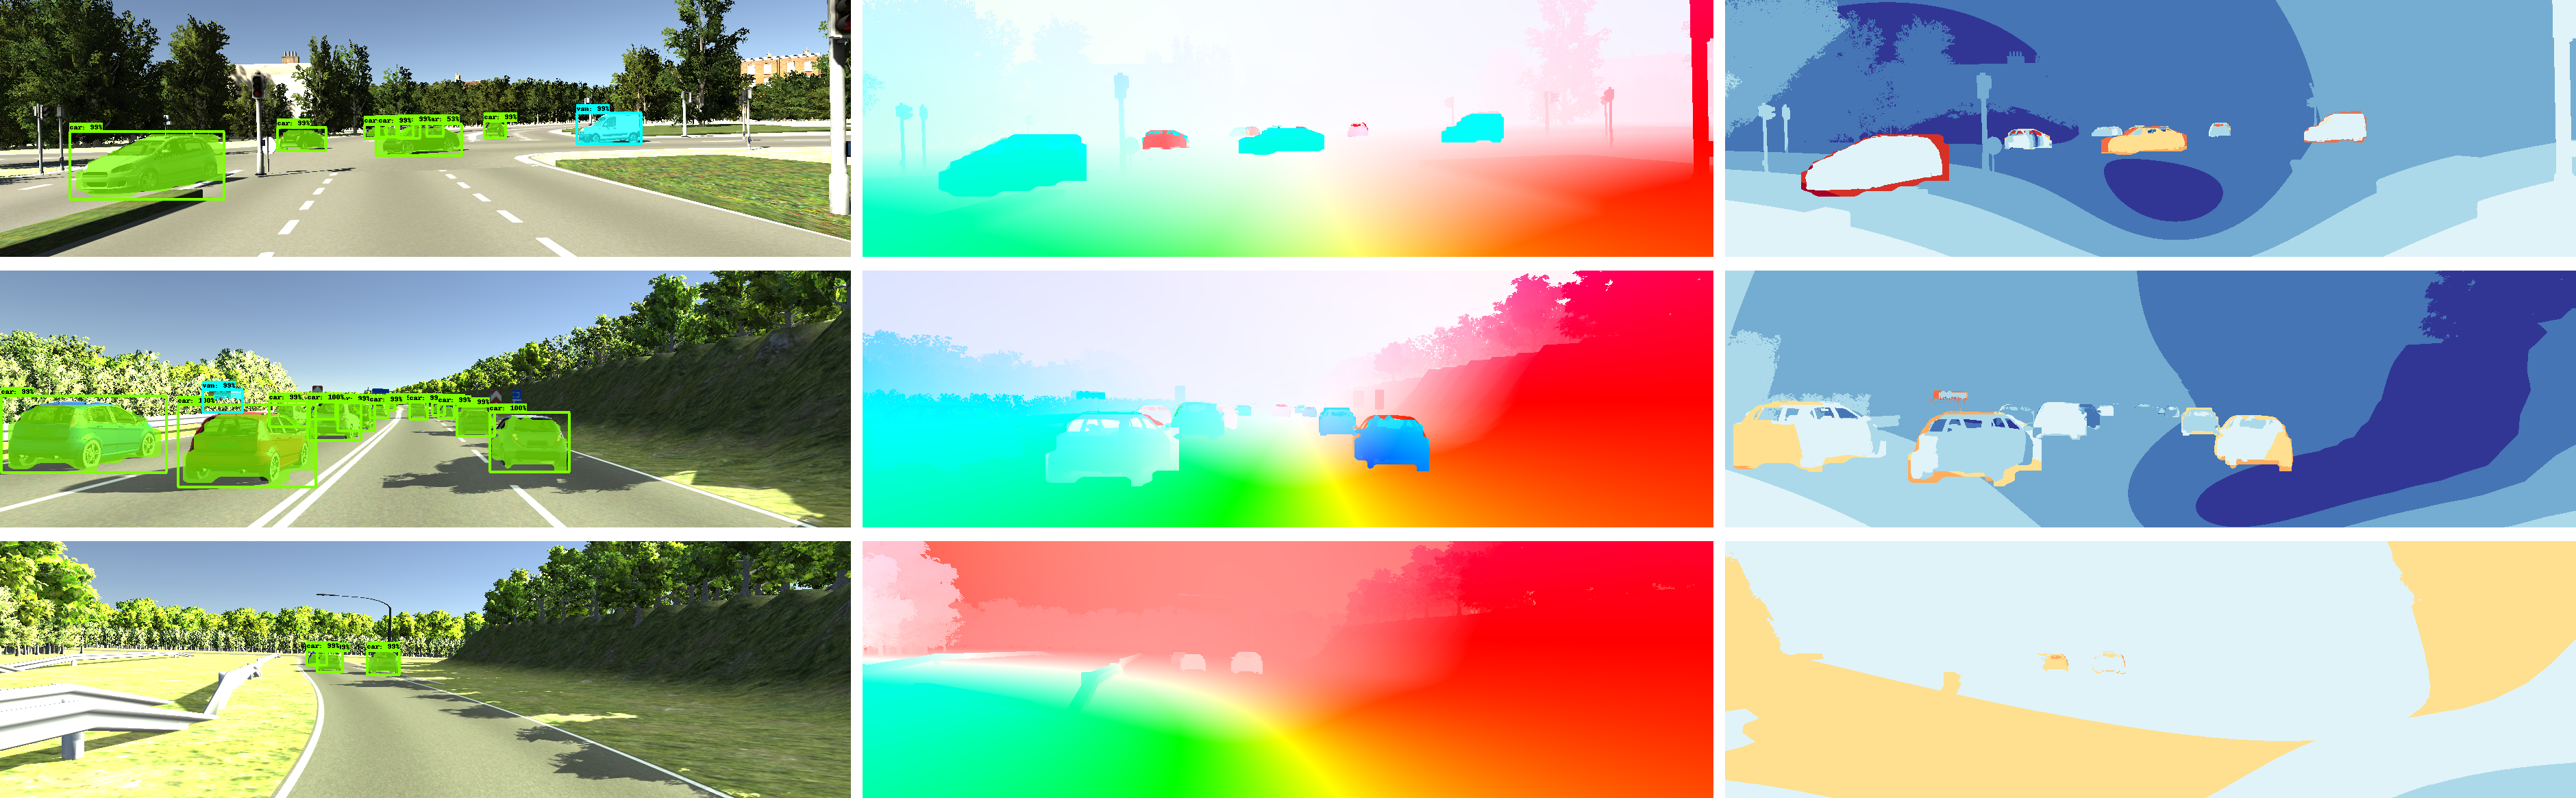
\includegraphics[width=\textwidth]{figures/vkitti_cam}
\caption{
Visualization of results with XYZ input, camera motion prediction and 3D motion supervision
with the ResNet (without FPN) architecture.
From left to right, we show the input image with instance segmentation results as overlay,
the estimated flow, as well as the flow error map.
The flow error map depicts correct estimates ($\leq 3$ px or $\leq 5\%$ error) in blue and wrong estimates in red tones.
}
\label{figure:vkitti}
\end{figure}

{
\begin{table}[t]
\centering
\begin{tabular}{@{}*{11}{c}@{}}
\toprule
\multicolumn{4}{c}{Network} & \multicolumn{3}{c}{Instance Motion Error} & \multicolumn{2}{c}{Camera Motion Error} &\multicolumn{2}{c}{Optical Flow Error} \\
  \cmidrule(lr){1-4}\cmidrule(lr){5-7}\cmidrule(l){8-9}\cmidrule(l){10-11}
FPN        & cam.       & sup. & XYZ         & $E_{R} [deg]$ & $E_{t} [m]$ & $E_{p} [m] $ & $E_{R}^{cam} [deg]$ & $E_{t}^{cam} [m]$ & AEE   & Fl-all \\\midrule
$\times$   & \checkmark & 3D   & \checkmark  & 0.4           & 0.49        & 17.06        & 0.1                 & 0.04              & 6.73  & 26.59\%    \\
\checkmark & \checkmark & 3D   & \checkmark  & 0.35          & 0.38        & 11.87        & 0.22                & 0.07              & 12.62 & 46.28\%    \\
$\times$   & $\times$   & 3D   & \checkmark  & ?             & ?           & ?            & -                   & -                 & ?     & ?    \%    \\
\checkmark & $\times$   & 3D   & \checkmark  & ?             & ?           & ?            & -                   & -                 & ?     & ?    \%    \\
  \midrule
$\times$   & \checkmark & flow   & \checkmark  & ?             & ?           & ?            & ?                   & ?                 & ?     & ?    \%    \\
\checkmark & \checkmark & flow   & \checkmark  & ?             & ?           & ?            & ?                   & ?                 & ?     & ?    \%    \\
$\times$   & $\times$   & flow   & \checkmark  & ?             & ?           & ?            & -                   & -                 & ?     & ?    \%    \\
\checkmark & $\times$   & flow   & \checkmark  & ?             & ?           & ?            & -                   & -                 & ?     & ?    \%    \\
  \bottomrule
\end{tabular}

\caption {
Comparison of network variants on the Virtual KITTI validation set.
AEE: Average Endpoint Error; Fl-all: Ratio of pixels where flow estimate is
wrong by both $\geq 3$ pixels and $\geq 5\%$.
Camera and instance motion errors are averaged over the validation set.
We optionally enable camera motion prediction (cam.),
replace the ResNet-50 backbone with ResNet-50-FPN (FPN),
or input XYZ coordinates into the backbone (XYZ).
We either supervise
object motions (sup.) with 3D motion ground truth (3D) or
with a 2D re-projection loss based on flow ground truth (flow).
Note that for rows where no camera motion is predicted, the optical flow
is composed using the ground truth camera motion and thus the flow error is
only impacted by the predicted 3D object motions.
}
\label{table:vkitti}
\end{table}
}
Figure \ref{figure:vkitti} visualizes instance segmentation and optical flow
results on the Virtual KITTI validation set.
Table \ref{table:vkitti} compares the performance of different network variants on the Virtual KITTI validation
set.

\subsection{Evaluation on KITTI 2015}
\todo{if there is enough time,
add evaluation (table + visualizations) of instance segmentation and composed optical flow on RGB-D frames from KITTI 2015 train}
